\section{Sprint een: Realiseren Peer to Peer netwerk}

\begin{table}[ht]
    \begin{tabular}{|p{0.3\textwidth}|p{0.65\textwidth}|}
      \hline
      \textbf{Scenarios} & UC03 - Connectie leggen deelnemer \\
      \hline
      & UC09 - Versturen bericht \\
      \hline
      \textbf{Componenten} & Node, Network \\
      \hline
    \end{tabular}
    \caption[Betrokken architectuur onderdelen implementatie Peer-to-Peer netwerk]{Betrokken scenarios en componenten bij de realisatie van het Peer-to-Peer netwerk.}
    \label{realisatie:p2p}
\end{table}

\begin{wrapfigure}[11]{r}{.5\textwidth}
    \begin{lstlisting}[
      language=Gherkin,
      caption={Scenario vertaald naar een Cucumber test suite.},
      label={testsuite:connect_to_participant},
      basicstyle=\footnotesize,
      captionpos=b
    ]
      Feature: Connect to participant
      As a user
      I want to connect to a participant
      So that I can communicate with the participant
  
      Scenario: Create connection
        Given there is no connection yet
        And I have entered the address
        When I press enter
        Then I should be connected with 
  
      Scenario: Create connection with unreachable address
        Given there is no connection yet
        And I have entered the address
        When I press enter
        Then I should receive a message "unreachable address"
    \end{lstlisting}
\end{wrapfigure}

Deze sprint staat in het teken van de basis van het Distributed Network, namelijk het opzetten van het netwerk. Een overzicht van de betrokken scenario's en componenten is te vinden in tabel \ref{realisatie:p2p}. Het eerste wat ik gedaan heb is het vertalen van de scenario naar een Cucumber test suite. Deze test suite zal gebruikt worden om te valideren dat de gerealiseerde functionaliteit voldoet aan de opgestelde criteria. In listing \ref{testsuite:connect_to_participant} is de opgestelde test suite te vinden voor de scenario ``Connectie leggen deelnemer''.

\subsection{Protocol}

In het vooronderzoek is er geleerd dat een \acrfull{P2P} netwerk centraal staat in het segment Distributed Network. Het \acrshort{P2P} netwerk kan gerealiseerd worden door gebruik te maken van twee mogelijke protocollen: het \acrfull{TCP} en het \acrfull{UDP}. Om hierin een keuze te maken is er een korte analyse gedaan over de aspecten van deze twee protocollen.

\subsubsection{Transmission Control Protocol} 

Het \acrfull{TCP} is het meest gebruikte protocol op het internet, het wordt namelijk gebruikt om data die benodigd is om een website te laden, te versturen. Een voordeel van \acrshort{TCP} is dat het protocol de garantie geeft dat data in de juiste volgorde ontvangen wordt. Het protocol wacht namelijk op bevestiging dat een \gls{packet} ontvangen is, alvorens een volgende \gls{packet} verstuurd word. Tevens zorgt dit ervoor dat data nooit corrupt raakt of verloren gaat.

\clearpage
\subsubsection{User Datagram Protocol}

Het \acrfull{UDP} werkt hetzelfde als \acrshort{TCP} alleen zit in dit protocol niet de controle of een \gls{packet} correct is aangekomen. \Glspl{packet} worden achter elkaar verstuurd zonder na te gaan of de ontvanger ze daadwerkelijk ontvangen heeft. Dit zorgt ervoor dat de overhead van het controleren niet aanwezig is, waardoor het sneller is als het \acrshort{TCP} protocol.

Omdat binnen een Blockchain implementatie garantie dat een transactie geregistreerd wordt zeer belangrijk is, zal er gebruik gemaakt worden van TCP/IP. De fail-safe mechaniek die in het protocol zit zal helpen om de Blockchain in een betrouwbare staat te houden.

\subsubsection{Selectie framework}

Aangezien het niet verstandig is om dit protocol zelf te realiseren ben ik op zoek gegaan naar frameworks die het \acrshort{TCP} protocol ondersteunen. Hierbij viel mijn oog al snel op het Netty framework. Netty is een client-server framework die het mogelijk maakt om snel en simpel een netwerk applicatie op te zetten die gebruik maakt van een \acrshort{TCP} socket server. De voorstaande reden voor het gebruik van Netty is de ondersteuning voor asynchroon programmeren, wat benodigd is om de hoge performance te behalen die nodig is voor een Blockchain implementatie. Daarnaast is Netty een de-facto standaard dat gebruikt wordt in prominente Java frameworks zoals Spring Boot, Google's GRPC en Minecraft.

\subsection{Ontwerpen}

Nu ik weet welk protocol gebruikt gaat worden voor het realiseren van het netwerk, heb ik een eerste draft gemaakt van het netwerk onderdeel dat conform de functionaliteiten van het Netty framework zijn. Het ontwerp is in fig. \ref{sprint_1:network} te zien. Alle componenten zijn modulair opgebouwd conform de afspraak die gemaakt is over de realisatie de Blockchain. Zo zijn de functionaliteiten geïsoleerd in desbetreffende componenten waardoor ze gemakkelijk verwisseld kunnen worden.

\clearpage

\begin{figure}[h]
    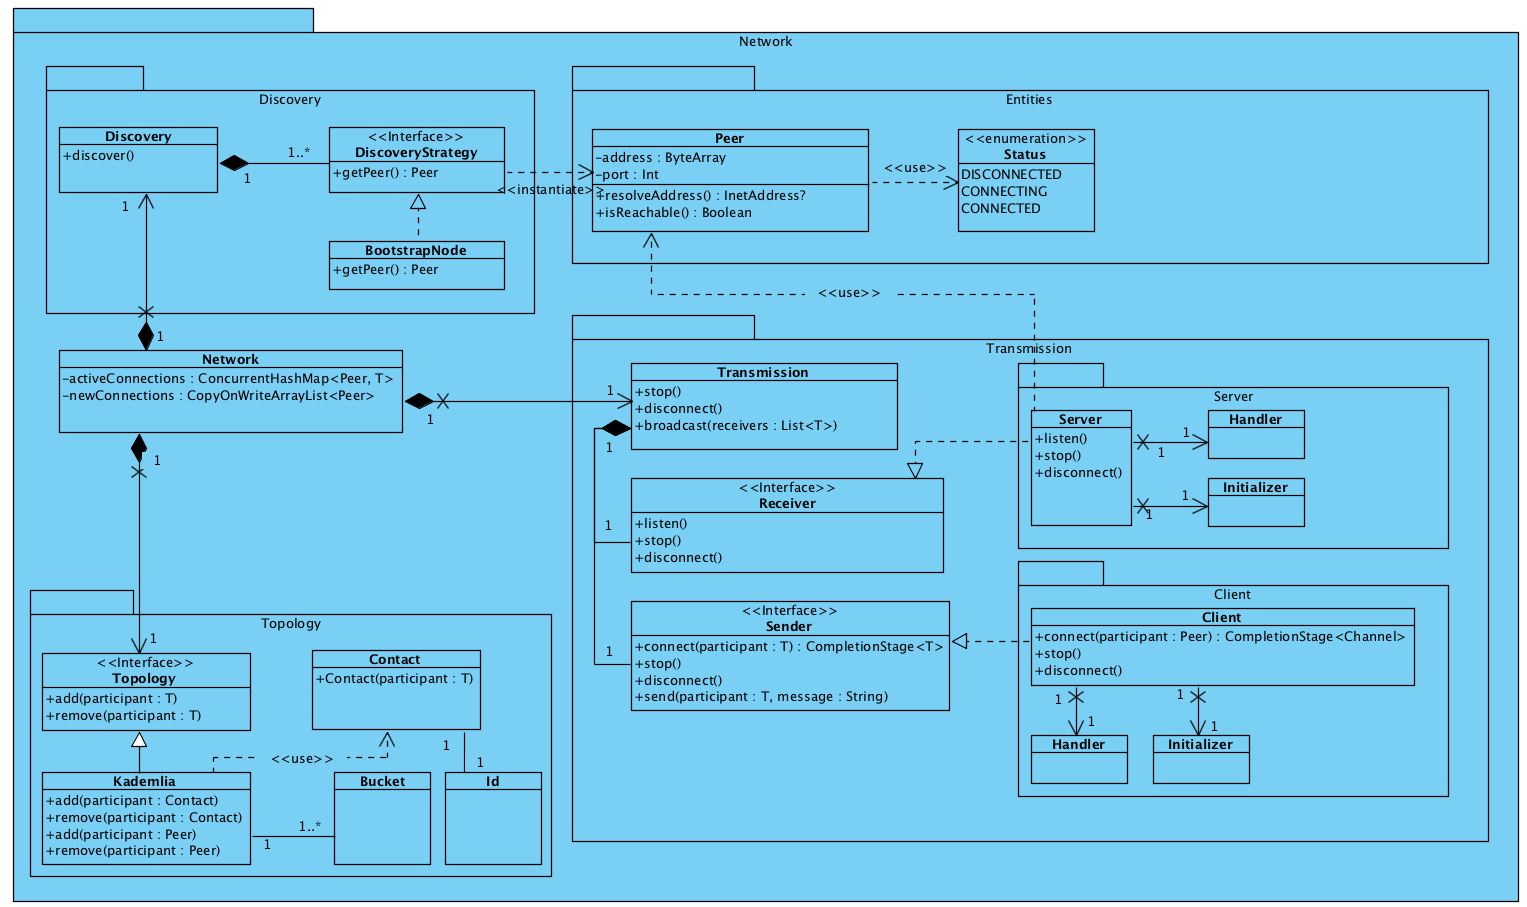
\includegraphics[width=\textwidth, keepaspectratio]{figures/network}
    \caption[Gedetailleerd overzicht Network component]{Gedetailleerd network component.}
    \label{sprint_1:network}
\end{figure}

\subsection{Versturen berichten}

Voor de tweede scenario ``Versturen bericht'' is het benodigd om data om te zetten naar een formaat dat gemakkelijk verstuurd kan worden over het \acrshort{P2P} netwerk. Een van de standaard technieken hiervoor is het omzetten van een entiteit naar bytes, door een proces genaamd serialisation. Dit is niet een van de meeste efficiënte manieren om data te versturen aangezien er een overhead is voor het omzetten en terugzetten van bytes naar entiteit en entiteit naar bytes. Om deze reden is er dan ook gezocht naar een efficiëntere manier om data te versturen. Hieronder zijn twee mogelijkheden beschreven die gebruikt kunnen worden op de \acrfull{JVM}. 

\begin{enumerate}
  \item \textbf{Java Serializable}
  \\ De standaard manier van het implementeren van serialisatie binnen Java. Door het implementeren van een interface op een klasse is het mogelijk om een object out-of-the-box te serialiseren. Wanneer er gebruik wordt gemaakt van complexere entiteiten dient de programmeur de serialisatie zelf te implementeren.
  \item \textbf{Protobuf}
  \\ Protocol buffers zijn Google's programmeertaal-neutrale implementatie van serialisatie. Door het eenmalig definiëren van de structuur door middel van een proto-bestand, is het mogelijk om via de library eenvoudig complexe entiteiten om te zetten naar bytes en van bytes naar entiteit. Een voordeel van Protobuf is dat het samenwerkt met alle talen die de library ondersteund. Op dit moment zijn dat Java, Python, Objective-C en C++ \citep{protobuf}.
\end{enumerate}

De keuze hierbij is gevallen op Protobuf om entiteiten binnen de Blockchain applicatie te serialiseren. Het voordeel van Protobuf is namelijk dat het samenwerkt met alle talen die de library ondersteund. Dit zorgt ervoor dat het serialisatieproces toekomstbestendig blijft.

\begin{wrapfigure}[16]{l}{0.4\textwidth}
    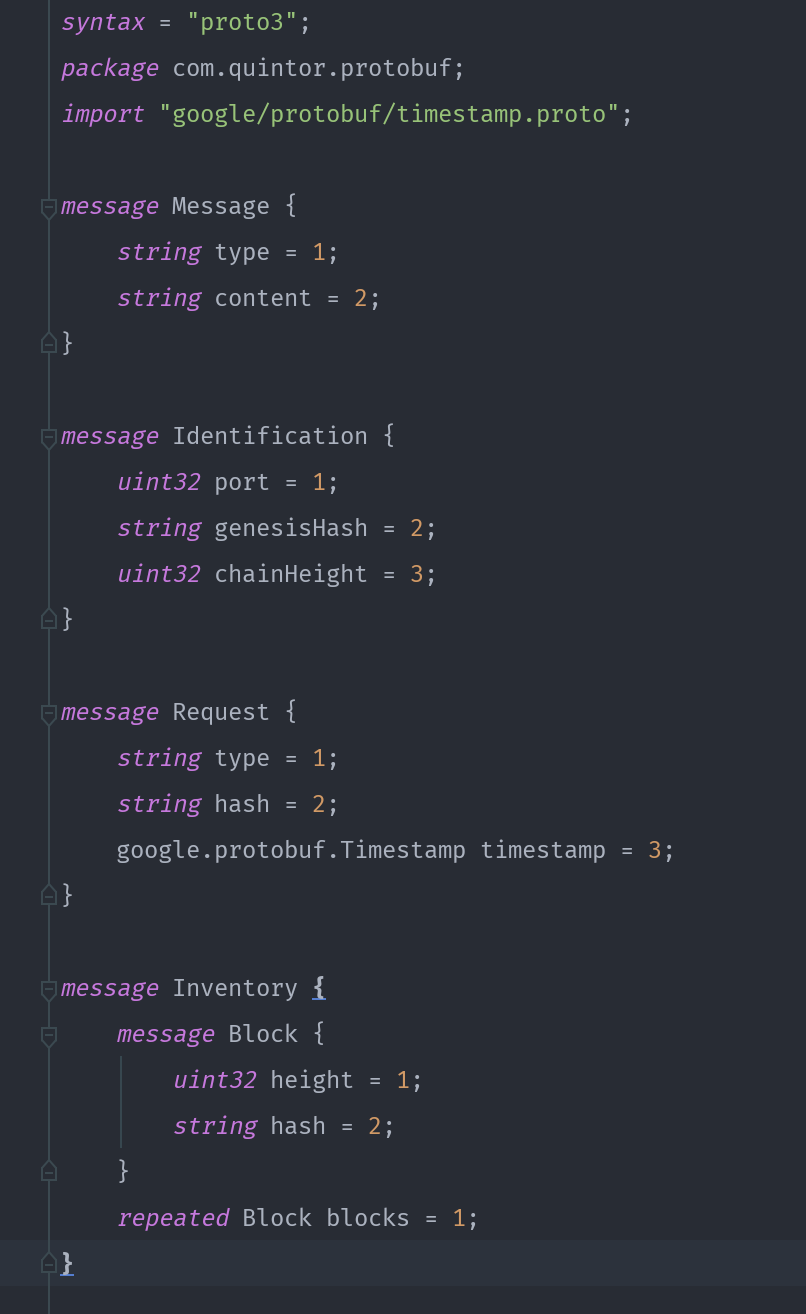
\includegraphics[width=0.4\textwidth, keepaspectratio]{figures/protobuf}
    \caption[Protobuf]{Opgesteld Protobuf bestand.}
    \label{sprint_1:protobuf}
\end{wrapfigure} 

In fig. \ref{sprint_1:protobuf} is het Protobuf bestand te zien dat opgesteld is om de berichtenstructuur van Bitcoin te implementeren. 

\subsection{Resultaat}

Aangezien mijn tijd beperkt was en de deze sprint in de laatste week gerealiseerd is ben ik over het algemeen tevreden met wat ik in deze sprint heb bereikt. Ik heb grotendeel van de architectuur opgezet en de basis van het \acrshort{P2P} netwerk gerealiseerd. Ook heb ik alvast een fundering neergezet voor het implementeren van de Protobuf entiteiten. Wel ben ik teleurgesteld dat ik niet verder ben gekomen met de realisatie van de functionaliteit. Daarnaast heb ik geen validaties kunnen doen door het uitvoeren van de opgestelde testen. 

